\documentclass[12pt, twoside]{article}

\usepackage{amsfonts}
%\usepackage[T1]{fontenc}
%\usepackage[ansinew]{inputenc}
\usepackage{amssymb}
\usepackage{amsthm}
\usepackage{amsmath}
\usepackage{dsfont}
\usepackage{natbib}
\setlength{\bibsep}{0pt plus 100ex}
\usepackage{url}
\usepackage{pdflscape}
\usepackage{pdfpages}
\usepackage{svg}
\usepackage[utf8]{inputenc}
\usepackage{graphicx}


\usepackage{enumitem}
%\usepackage[german,  onelanguage, linesnumbered]{algorithm2e}
\usepackage{placeins}
\usepackage{a4}
\usepackage[a4paper, ]{geometry}
\geometry{
 a4paper,
 right=30mm,
 left=30mm,
 top=30mm,
 }

% For tables
\usepackage{tabularx}
\usepackage{multirow}
\usepackage{pbox}

% \usepackage{color}

\widowpenalty = 5000
\clubpenalty = 5000


\newcommand{\Prob}{\mathbb{P}}
\newcommand{\V}{\mathbb{V}}
\newcommand{\Cov}{\text{Cov}}
\newcommand{\E}{\mathbb{E}}
\newcommand{\R}{\mathbb{R}}
\newcommand{\1}{\mathbb{1}}
\newcommand{\LL}{\mathcal{L}}
\newcommand{\F}{\mathcal{F}}
\newcommand{\iid}{\overset{\text{iid}}{\sim}}
\newcommand{\SUM}{\sum_{i=1}^n}
\newcommand{\PROD}{\prod_{i=1}^n}



\begin{document}

\begin{titlepage}

    \newcommand{\HRule}{\rule{\linewidth}{0.5mm}} % Defines a new command for the horizontal lines, change thickness here

    \center % Center everything on the page
 
    %----------------------------------------------------------------------------------------
    %	HEADING SECTIONS
    %----------------------------------------------------------------------------------------
    
\includegraphics[scale = 0.22]{campus-seal.jpg}\\[0.5cm]
    
     \textsc{\large University of California, los Angeles}\\[0.2cm] % Minor heading such as course title
     \textsc{\large Department of Statistics}\\[0.5cm]
    %----------------------------------------------------------------------------------------
    %	TITLE SECTION
    %----------------------------------------------------------------------------------------

    \HRule \\[0.4cm]
    { \huge \bfseries Metric Entropy}\\[0.2cm] % Title of your document
    \HRule \\[0.4cm]
    \textsc{\large Subtitle}\\[2.0 cm]
 
    %----------------------------------------------------------------------------------------
    %	AUTHOR SECTION
    %----------------------------------------------------------------------------------------
    
    	\hspace{1cm}
    \begin{minipage}{0.4\textwidth}
    \begin{flushleft} \large
    \emph{Authors:}\\
        Melody \textsc{Huang} \\
        Conor \textsc{Kresin} \\
        Thomas \textsc{Maierhofer} % Your name
    \end{flushleft}
    \end{minipage}
    ~
    \begin{minipage}{0.4\textwidth}
    \begin{flushright} \large
    \emph{Stats 200C:} \\
    Spring Quarter 2019, \\
    Prof. Arash Amini \\ % Supervisor's Name 
    \text{ }
    \end{flushright}
    \end{minipage}\\[2cm]
    
    \large{
    Final Project Report
    } \\[2cm]
    
    {\large March 22, 2019}\\[2cm] % Date, change the \today to a set date if you want to be precise

    %----------------------------------------------------------------------------------------

    \vfill % Fill the rest of the page with whitespace

\end{titlepage}

%\newpage
%\hspace{5cm}
%\newpage

\pagenumbering{roman}
\tableofcontents 
\clearpage

\begin{abstract}
TODO
\end{abstract}
\clearpage
\pagenumbering{arabic}

\section{Background}

\subsection{$p$ Norms for Vectors}
This section formally introduces $p$ norms with a focus on the special cases $ p = 0, 1, 2, \infty$.
The $p$ norm of a vector $x \in \R^d$ is denoted as $||x||_p$ and defined as
$$||x||_p = \left(\sum_{i = 1}^d |x_i|^p \right)^{1/p},$$
where $|x_i| = \text{sign}(x_i)x_i$ denotes the absolute value.
%
The most important special cases include the $0$ norm is which counting the non-zero entries in $x$,
$$||x||_0 = \sum_{i = 1}^d \1\{x_i \neq 0\},$$
the $1$ norm, a.k.a.\ city-block norm,
$$||x||_1 = \sum_{i = 1}^d |x_i|,$$
the $2$ norm, a.k.a.\ Euclidean norm,
$$||x||_2 = \sqrt{\sum_{i = 1}^d x_i^2},$$
and the $\infty$ norm, a.k.a. maximum norm,
$$||x||_\infty = \max_{i = 1, \ldots, d} |x_i|.$$

A unit ball for a norm $||\cdot||$ contains all points with distance $1$ around the origin, i.e. all points $\{x: ||x|| = 0\}$. The unit balls for the $0, 1, 2,$ and $\infty$ norm in $\R^2$ are depicted in Figure~\ref{fig:input}. Note that the volume of the unit balls increases in $p$.
\begin{figure}[ht]
    \centering
    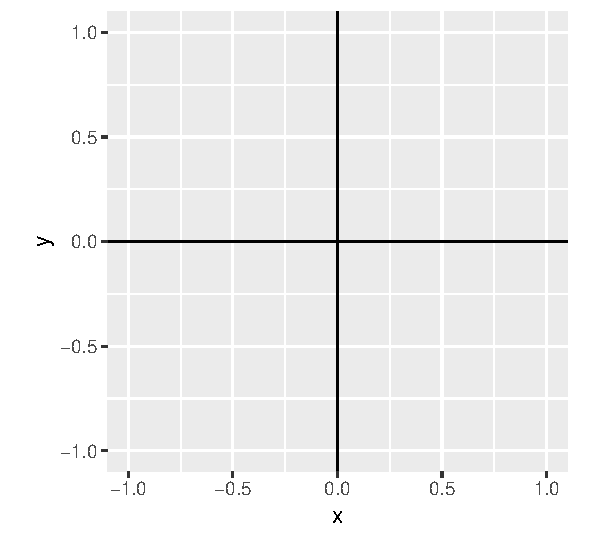
\includegraphics[width=0.49\textwidth]{plots/unit_circle_0.pdf}
    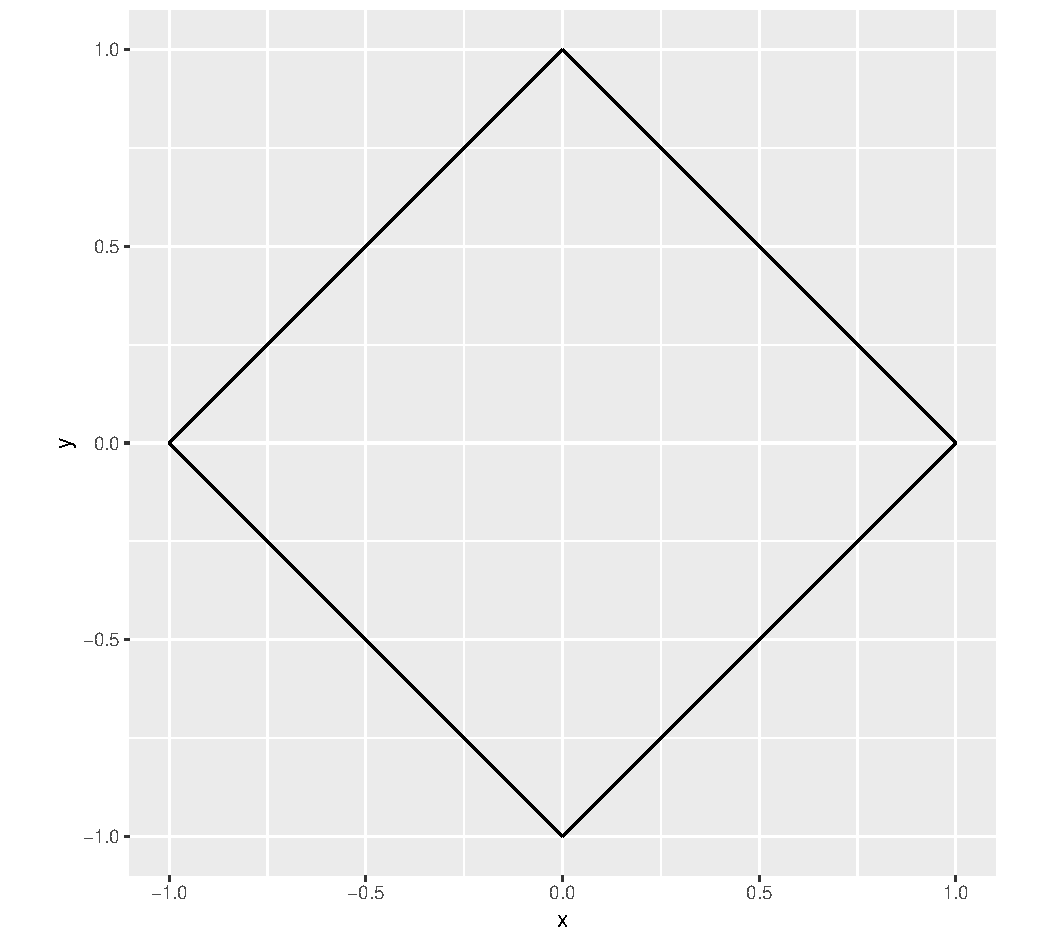
\includegraphics[width=0.49\textwidth]{plots/unit_circle_1.pdf}
    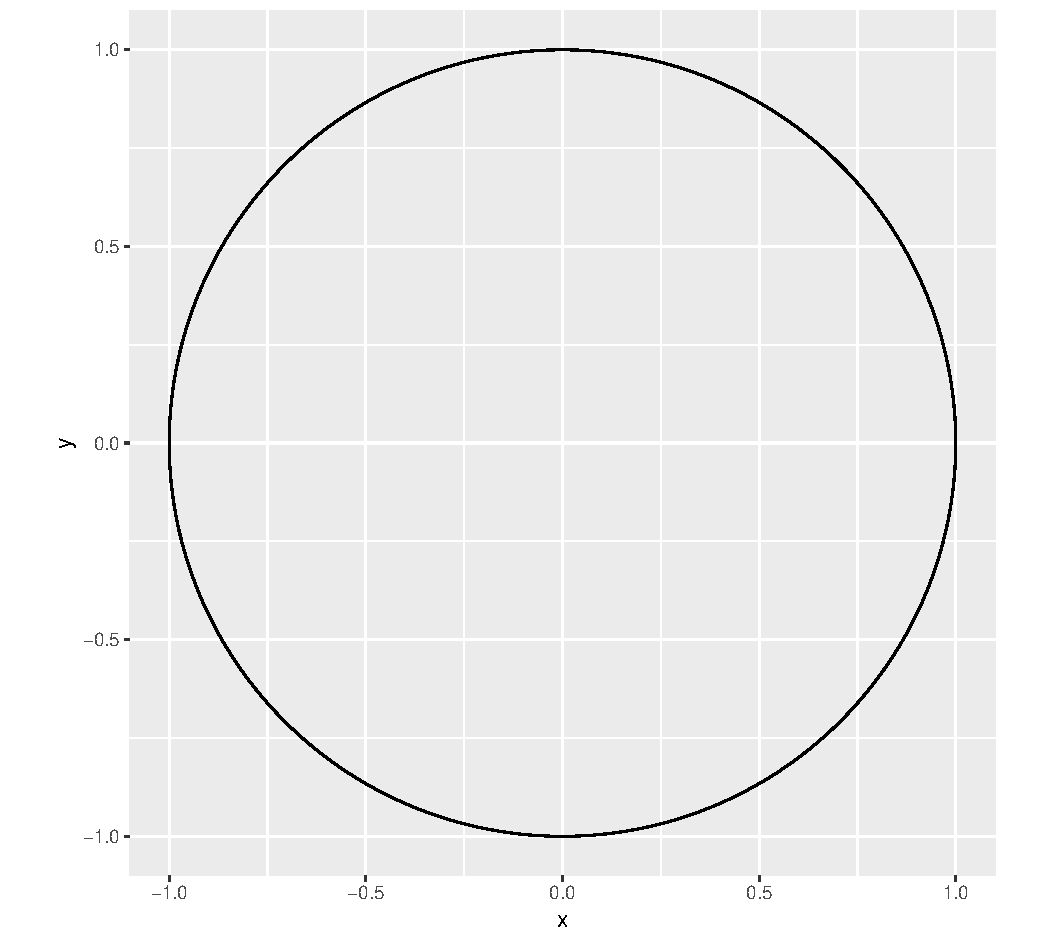
\includegraphics[width=0.49\textwidth]{plots/unit_circle_2.pdf}
    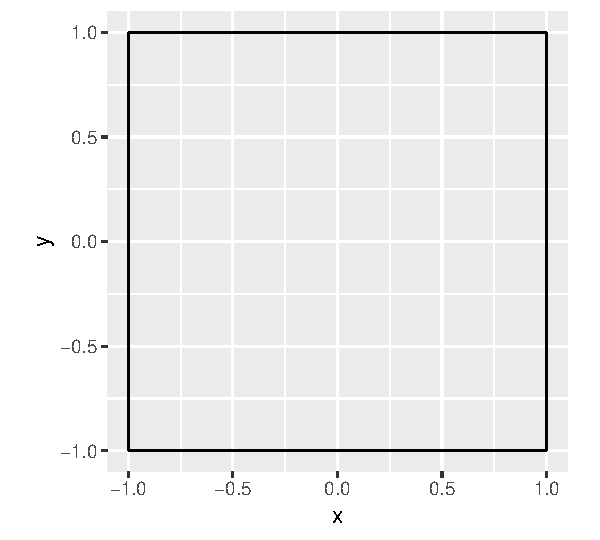
\includegraphics[width=0.49\textwidth]{plots/unit_circle_inf.pdf}
    \caption{Unit balls in $\R^2$ of the $0$ (top left), $1$ (top right), $2$ (bottom left), an $\infty$ norm (bottom right).}
    \label{fig:input}
\end{figure}


\subsection{Entropy}
Entropy measures how far from deterministic a random variable is, i.e. entropy quantifies a random variables diversity, uncertainty or randomness. 
A random variable with entropy zero is deterministic, an increasing value  means that it is more and more unpredictable.
This section introduces the Shannon entropy and R\'enyi entropy for discrete random variables, the case of continuous random variables follows directly by replacing sums with intergrals.
    
\subsubsection{Shannon Entropy}
Let $ X $ be a discrete random variable taking values in the set $ \{x = x_1, x_2, \ldots, x_n \} $ with probabilities $ \{p = p_1, p_2, \ldots, p_n \} $. The Shannon entropy $ H(X) $ is defined as 

\begin{equation}\label{Shannon1}
    H(X) = H_1(X) = - \sum_{i = 1} ^ n p_i \log_2 p_i,
\end{equation}
and obtains its maximum value for the uniform distribution
$$p_i = \frac{1}{n} \forall i.$$
Considerations of continuity lead to the adoption of the convention, $ 0 \log 0  = 0 $.

\subsubsection{R\'enyi Entropy}
The R\'enyi entropy of order $ q $, $ q  \geq 0 $ and $ q \neq 1 $, of a discrete random variable $ X $ taking $ n $ values with probabilities $ p_1, \ldots, p_n $, is defined as,
\begin{equation}
        H_q(X) = 
        \frac{1}{1 - q} \log \left( \sum_{i=1}^n p_i ^ {q} \right)
        = \frac{1}{1 - q} \log \| p \|_q^q,  
\end{equation}
using the $ p $-norm of order $ q $ of $ x  \in \R ^ n $  which is defined as   
$$ \| x \|_q = \left( \sum_{i=1}^n |x_i|^q \right)^{1/q}, \textrm{ for } q \geq 1 \in \R. $$

The most important special cases are $q = 0$ (count norm) for the max-entropy,
$$ 
H_0(X) = \lim_{q \to 0} \frac{1}{1 - q} \log \| p \|_q^q =  \log |X|,
$$
which is the logarithm of the cardinality of $X$,
$ q = 1 $ (Manhattan norm) for the Shannon entropy \footnote{or more precisely $\lim_{q \to 1} H_q(X) = H(X)$}, see Equation~\eqref{Shannon1},  $ q = 2 $ (Euclidean norm)  for the quadratic entropy or collision entropy, 
$$ 
H_2(X) = \frac{1}{1 - 2} \log \| p \|_2^2 = \log \sum_{i} p_i^2,
$$
and $q = \infty$ (maximum norm) used in the Min entropy,
$$ 
H_\infty(X) = \lim_{q \to \infty} \frac{1}{1 - q} \log \| p \|_q^q = \log \max_{i} p_i,
$$
This means that the parameter $ q $ changes the way the shape of the distribution influences the entropy by designating the norm being used. Different parameters $q$ make the R\'enyi entropy more or less sensitive to certain characteristics of the probability distributions.
Note that the R\'enyi  entropy is monotonically decreasing in $q$, as the $q$ norms are monotonically decreasing and the $\log$ is a monotonic transformation. 

\subsection{Example: R\'enyi Entropy of Dirichlet distribution}
The R\'enyi entropy of a $3$ dimensional Dirichlet with parameter $\alpha$ distributed random variable $X$ is given as
$$H_q(X) = \frac{1}{1 - q} \log(\frac{\Gamma^q(\alpha_1 + \alpha_2 + \alpha_3) \Gamma(q \alpha_1 - q + 1) \Gamma(q \alpha_2 - q + 1) \Gamma(q \alpha_3 - q + 1)}{\Gamma(q (\alpha_1 + \alpha_2 + \alpha_3 - 3) + 3) (\Gamma(\alpha_1) \Gamma(\alpha_2) \Gamma(\alpha_3))^q}).$$

For a given $\alpha \in \R^3,$ the Dirichlet distribution defines a distribution on $\R^2,$ as $\sum_{i = 1}^3 x_i = 1$. The distribution for $\alpha = (3, 5, 3)$ is visualized in Figure~\ref{dir_dist}.



Using this formula, we can compute the R\'enyi entropy for a given parameter $q$ in Table~\ref{tab:renyi_ent}.
\begin{table}[]
\caption{R\'enyi of a 3 dimensional Dirichlet with parameter $\alpha = (3, 5, 3)$ distributed random variable for varying $q$.}
\begin{tabular}{l|lllllll}
q    & 0.01   & 0.5    & 0.99                       & 1      & 1.01   & 2      & 10     \\ \hline
$H_q$ & -0.714 & -1.232 & \multicolumn{1}{r}{-1.439} & -1.442 & -1.445 & -1.645 & -1.991
\end{tabular}
\label{tab:renyi_ent}
\end{table}


%%%%%%%%%%%%%%%%%%%%%%%%%%%%%%%%%%%%%%%%%%%%%%%%%%%%%%%%%%%%%%%%%%%%%
\section{Metric Entropy}
Metric entropy quantifies the size of a set $T$. This task is superficially unrelated to the concept of entropy, but after closer inspections similarities become apparent.

\subsection{Covering and Packing}


%%%%%%%%%%%%%%%%%%%%%%%%%%%%%%%%%%%%%%%%%%%%%%%%%%%%%%%%%%%%%%%%%%%%%
\clearpage
\bibliographystyle{dcu} 
{\bibliography{bibliography.bib}}
\nocite{maierhoferCoFD}

%%%%%%%%%%%%%%%%%%%%%%%%%%%%%%%%%%%%%%%%%%%%%%%%%%%%%%%%%%%%%%%%%%%%%
% appendix

\end{document}